%%%%%%%%%%%%%%%%%%%%%%%%%%%%%%%%%%%%%%%%%%%%%%%%%%%%%%%%%%%%%%%%%%%%%%%%%%%%%%%%%%%%%%%%%%%%%%%%%%%%%%%%%%%%%%%%%%%%%%%%%%%%%%%%%%%%%%%%%%%%%%%%%%%%%%%%%%%
% This is just an example/guide for you to refer to when submitting manuscripts to Frontiers, it is not mandatory to use Frontiers .cls files nor frontiers.tex  %
% This will only generate the Manuscript, the final article will be typeset by Frontiers after acceptance.   
%                                              %
%                                                                                                                                                         %
% When submitting your files, remember to upload this *tex file, the pdf generated with it, the *bib file (if bibliography is not within the *tex) and all the figures.
%%%%%%%%%%%%%%%%%%%%%%%%%%%%%%%%%%%%%%%%%%%%%%%%%%%%%%%%%%%%%%%%%%%%%%%%%%%%%%%%%%%%%%%%%%%%%%%%%%%%%%%%%%%%%%%%%%%%%%%%%%%%%%%%%%%%%%%%%%%%%%%%%%%%%%%%%%%

%%% Version 3.4 Generated 2018/06/15 %%%
%%% You will need to have the following packages installed: datetime, fmtcount, etoolbox, fcprefix, which are normally inlcuded in WinEdt. %%%
%%% In http://www.ctan.org/ you can find the packages and how to install them, if necessary. %%%
%%%  NB logo1.jpg is required in the path in order to correctly compile front page header %%%

\documentclass[utf8]{frontiersSCNS} % for Science, Engineering and Humanities and Social Sciences articles
\usepackage{url,hyperref,lineno,listings,microtype,subcaption}
\usepackage[onehalfspacing]{setspace}

% Automatic formatting of SI units
\usepackage[binary-units,separate-uncertainty=true]{siunitx}

\linenumbers


\lstset{language=C++,showstringspaces=false,basicstyle=\tiny,upquote=true,identifierstyle=\ttfamily\color{black}}

% Leave a blank line between paragraphs instead of using \\


\def\keyFont{\fontsize{8}{11}\helveticabold }
\def\firstAuthorLast{Knight and Nowotny} %use et al only if is more than 1 author
\def\Authors{James C Knight\,$^{1,*}$, Anton Komissarov, Thomas Nowotny\,$^{1}$}
\def\Address{$^{1}$Centre for Computational Neuroscience and Robotics, School of Engineering and Informatics, University of Sussex, Brighton, United Kingdom }
\def\corrAuthor{James C Knight}
\def\corrEmail{J.C.Knight@sussex.ac.uk}

\begin{document}
\onecolumn
\firstpage{1}

\title[PyGeNN]{PyGeNN: A Python library for GPU-enhanced neural networks} 

\author[\firstAuthorLast ]{\Authors} %This field will be automatically populated
\address{} %This field will be automatically populated
\correspondance{} %This field will be automatically populated

\extraAuth{}% If there are more than 1 corresponding author, comment this line and uncomment the next one.
%\extraAuth{corresponding Author2 \\ Laboratory X2, Institute X2, Department X2, Organization X2, Street X2, City X2 , State XX2 (only USA, Canada and Australia), Zip Code2, X2 Country X2, email2@uni2.edu}


\maketitle


\begin{abstract}

%%% Leave the Abstract empty if your article does not require one, please see the Summary Table for full details.
\section{}
For full guidelines regarding your manuscript please refer to \href{http://www.frontiersin.org/about/AuthorGuidelines}{Author Guidelines}.

As a primary goal, the abstract should render the general significance and conceptual advance of the work clearly accessible to a broad readership. References should not be cited in the abstract. Leave the Abstract empty if your article does not require one, please see \href{http://www.frontiersin.org/about/AuthorGuidelines#SummaryTable}{Summary Table} for details according to article type. 


\tiny
 \keyFont{ \section{Keywords:} keyword, keyword, keyword, keyword, keyword, keyword, keyword, keyword} %All article types: you may provide up to 8 keywords; at least 5 are mandatory.
\end{abstract}

\section{Introduction}
A wide range of spiking neural network~(SNN) simulators are available, each with their own niche. 
NEST~\citep{Gewaltig2007} is widely used for large-scale point neuron simulations on distributed computing systems; NEURON~\citep{carnevale2006neuron} and Arbor~\citep{Akar2019} specialise in the simulation of complex multi-compartmental models; and CARLsim~\citep{Chou2018} and GeNN~\citep{Yavuz2016} use Graphics Processing Units~(GPUs) to accelerate point neuron models.
For performance reasons, many of these simulators are written in C++ and, especially amongst the older simulators, users describe their models either using a Domain-Specific Language~(DSL) or directly in C++.
For programming language purists, a DSL may be an elegant way of describing an SNN network model and, for simulator developers, not having to add bindings to another language is convenient.
However, both choices act as a barrier to potential users.
Therefore, with both the computational neuroscience and machine learning communities gradually coalescing towards a Python-based ecosystem with a wealth of mature libraries for scientific computing~\citep{Hunter2007,VanDerWalt2011,Millman2011}, exposing spiking neural network simulators to Python seems a pragmatic choice.
NEST~\citep{Eppler2009}, Neuron~\citep{Hines2009} and CARLsim~\citep{Balaji2020} have all taken this route and now offer a Python interface.
Furthermore, newer simulators such as Arbor and Brian2~\citep{Stimberg2019} have been designed from the ground up with a Python interface.

While we have recently demonstrated some very competitive performance results~\citep{Knight2020} using our GeNN simulator~(Yavuz2016), it has not been usable directly from Python.
GeNN can already be used as a backend for the Python-based Brian2 simulator~\citep{Stimberg2019} but, while Brian2GeNN~\citep{Stimberg2020} allows Brian2 users to harness the performance benefits GeNN provides, it is not possible to expose all of GeNN's unique features to Python through the Brian2 API.
Specifically, GeNN not only allows users to easily define their own neuron and synapse models but, also `snippets' for offloading the potentially costly initialisation of model parameters and connectivity onto the GPU.
Additionally, GeNN  provides a lot of freedom for users to integrate their own code into the simulation loop.
In this paper we describe the implementation of PyGeNN -- a Python package which aims to expose the full range of GeNN functionality with minimal performance overheads.
We then demonstrate this performance using two large-scale models from the literature.

\begin{figure}[h!]
    \begin{center}
        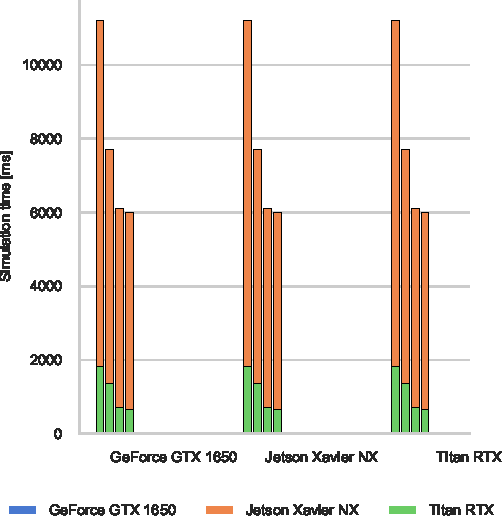
\includegraphics{figures/microcircuit_overheads.pdf}
    \end{center}
    \caption{}\label{fig:microcircuit_overheads}
\end{figure}

\section{Materials and Methods}
\subsection{GeNN}
GeNN~\citep{Yavuz2016} is a library for generating CUDA code for the simulation of spiking neural network models.
GeNN handles much of the complexity of using CUDA directly as well as automatically performing device-specific optimizations so as to to maximize performance.

GeNN consists of a main library -- implementing the API used to define models as well as the generic parts of the code generator -- and an additional library for each backend (currently there is a reference C++ backend for generating CPU code and a CUDA backend. An OpenCL backend is under development).
Users describe their model by implementing a \lstinline{modelDefinition} function within a C++ file. For example, a model consisting of a single leaky integrate-and-fire neurons might be defined as follows:
%
\begin{lstlisting}[language=C++]
void modelDefinition(ModelSpec &model)
{
    model.setDT(1.0);
    model.setName("example");
    
    NeuronModels::LIF::ParamValues params(0.25, 10.0, 0.0, 0.0, 
                                          20.0, 2.0, 0.5);
    NeuronModels::LIF::VarValues init(5.0, 0.0);
    
    model.addNeuronPopulation<NeuronModels::LIF>("Pop", 1, params, init);
}
\end{lstlisting}
%
The \emph{genn-buildmodel} tool is then used to compile this file; link it against the main GeNN library and the desired backend library; and finally run the resultant executable to generate the source code required to build a simulation dynamic library (a .dll file on Windows or a .so file on Linux and Mac).
Typically, this dynamic library is then statically linked against a simulation loop provided by the user, in this case one which simply prints the neuron's membrane voltage every timestep:
%
\begin{lstlisting}[language=C++]
#include "example_CODE/definitions.h"

int main()
{
  allocateMem();
  initialize();
  initializeSparse();

  while(t < 100.0f) {
     stepTime();
     pullVPopFromDevice();
     std::cout << t << "," << VPop[0] << std::endl;
  }
  return EXIT_SUCCESS;
}
\end{lstlisting}
%
Alternatively, the dynamic library can be dynamically loaded by the users simulation code.
Using this approach, an equivalent simulation loop could be implemented as follows using the \lstinline{SharedLibraryModel} helper class supplied with GeNN:
%
\begin{lstlisting}[language=C++]
#include "sharedLibraryModel.h"

int main()
{
  SharedLibraryModel<float> model("./", "example");
  model.allocateMem();
  model.initialize();
  model.initializeSparse();

  float *vPop = model.getScalar<float>("VPop");
  while(model.getTime() < 100.0f) {
     model.stepTime();
     model.pullVarFromDevice("Pop", "V");
     std::cout << model.getTime() << "," << vPop[0] << std::endl;
  }
  return EXIT_SUCCESS;
}
\end{lstlisting}
%
This second approach is key to the approach we use to implement PyGeNN.

\subsection{SWIG}
agaga

\subsection{PyGeNN}
agasg

\subsection{Cortical microcircuit model}
sfasfas

\subsection{Random balanced network HPC benchmark model}
aaaf

\section{Results}
asfgaf

\subsection{Cortical microcircuit model performance}
Figure~\ref{fig:microcircuit_overheads} shows the simulation times for the full-scale microcircuit mode on a representative selection of NVIDIA GPU hardware:
%
\begin{itemize}
    \item Jetson Xavier NX -- a low-power embedded system with \SI{8}{\giga\byte} of shared memory.
    \item GeForce GTX 1650 -- a low-end desktop GPU with \SI{4}{\giga\byte} of dedicated memory.
    \item Titan RTX -- a high-end workstation GPU with \SI{24}{\giga\byte} of dedicated memory.
\end{itemize}
%
As one might predict, the Jetson Xavier NX is slower than the two desktop GPUs.
However, considering that it only consumes a maximum of \SI{15}{\watt} compared to \SI{75}{\watt} or \SI{320}{\watt} for the GeForce GTX 1650 and Titan RTX respectively, it performs impressively.
The time taken to actually simulate the models (`Neuron simulation' and `Synapse simulation') are the same when using Python and C++ as all GeNN optimisation options are exposed to PyGeNN.
However, both the PyGeNN and C++ simulations spend a significant amount of every simulation step copying spike data off the device and storing it in a suitable data structure (`Overhead').
Because Python is an interpreted language, such operations are inherantly slower -- this is particularly noticable on devices with a slower CPU such as the Jetson Xavier NX.
When the spike recording system is used, spike data is kept in GPU memory until the end of the simulation and this overhead is reduced by around a factor of 10.
This now means that, on the high-end desktop GPU, this simulation now runs faster than real-time -- previously only achievable using a specialised neuromorphic system~\citep{Rhodes2019}.

\section{Discussion}
discuss!
\begin{itemize}
    \item PyGeNN as an intermediate layer - PyNN, ML
\end{itemize}

\section*{Conflict of Interest Statement}
The authors declare that the research was conducted in the absence of any commercial or financial relationships that could be construed as a potential conflict of interest.

\section*{Author Contributions}
JK and TN wrote the paper.
TN is the original developer of GeNN.
AK was the original developer of PyGeNN.
JK is currently the primary developer of both GeNN and PyGeNN and was responsible for implementing the spike recording system.
JK performed the experiments and the analysis of the results that are presented in this work.

\section*{Funding}
This work was funded by the EPSRC (Brains on Board project, grant number EP/P006094/1).

\section*{Acknowledgments}
This is a short text to acknowledge the contributions of specific colleagues, institutions, or agencies that aided the efforts of the authors.

\section*{Data Availability Statement}
The datasets [GENERATED/ANALYZED] for this study can be found in the [NAME OF REPOSITORY] [LINK].
% Please see the availability of data guidelines for more information, at https://www.frontiersin.org/about/author-guidelines#AvailabilityofData

\bibliographystyle{frontiersinSCNS_ENG_HUMS} % for Science, Engineering and Humanities and Social Sciences articles, for Humanities and Social Sciences articles please include page numbers in the in-text citations
\bibliography{pygenn}

\end{document}
